\documentclass{article}
\usepackage[left=0.5in,top=0.5in,right=0.5in,bottom=0.5in]{geometry}
\usepackage[dvipsnames]{xcolor}
\usepackage[english]{babel}
\usepackage[utf8]{inputenc}
\usepackage{graphicx}
\usepackage{
  amssymb,
  amsmath,
  amsthm,
  latexsym
}
\graphicspath{{./images/}}
\title{Comparing Two Mosses Lab Report}
\author{Philip Kim}
\date{\today}
\begin{document}
\maketitle
\begin{table}[h!]
  \begin{center}
    \caption{Scleropodium obtusifolium}
    \begin{tabular}{|c|c|c|}\hline
      Length & Width & W:L \\ \hline
      2.36 & 1.62 & 0.6864 \\ \hline
      2.67 & 1.65 & 0.6180 \\ \hline
      2.95 & 1.87 & 0.6339 \\ \hline
      2.16 & 1.29 & 0.5972 \\ \hline
      1.96 & 1.29 & 0.6582 \\ \hline
      2.82 & 1.76 & 0.6241 \\ \hline
      2.64 & 1.67 & 0.6326 \\ \hline
      2.97 & 1.9 & 0.6397 \\ \hline
      2.57 & 1.53 & 0.5953 \\ \hline
      2.67 & 1.8 & 0.6742 \\ \hline
      2.21 & 1.47 & 0.6652 \\ \hline
      2.91 & 1.91 & 0.6564 \\ \hline
      2.08 & 1.31 & 0.6298 \\ \hline
      2.54 & 1.62 & 0.6378 \\ \hline
      2.35 & 1.44 & 0.6128 \\ \hline
    \end{tabular}
  \end{center}
  \begin{center}
    \begin{equation}
      \begin{split}
        n &= 15 \\
        \overline{x} &= \frac{x_1 + x_2 + \cdots + x_n}{n} \\
        \sigma_{x} &= \sqrt{\frac{{|x_1 - \overline{x}|}^2 + {|x_2 - \overline{x}|}^2 + \cdots + {|x_n - \overline{x}|}^2}{n-1}} \\
        \epsilon_{x} &= \frac{\sigma_{x}}{\sqrt{n}} \\
        \overline{W:L} &= 0.6374 \\
        \sigma_{W:L} &= 0.0267 \\
        \epsilon_{W:L} &= 0.0069 \\
      \end{split}
    \end{equation}
  \end{center}
\end{table}
\newpage
\begin{table}[h!]
  \begin{center}
    \caption{Scleropodium possible new-sp}
    \begin{tabular}{|c|c|c|}\hline
      Length & Width & W:L \\ \hline
      1.82 & 1.65 & 0.9066 \\ \hline
      2.41 & 2.21 & 0.9170 \\ \hline
      2.03 & 1.77 & 0.8719 \\ \hline
      2.16 & 2 & 0.9259 \\ \hline
      2.18 & 1.96 & 0.8991 \\ \hline
      1.95 & 1.86 & 0.9538 \\ \hline
      2.61 & 2.25 & 0.8621 \\ \hline
      2.41 & 2.11 & 0.8755 \\ \hline
      2.46 & 2.1 & 0.8537 \\ \hline
      1.86 & 1.75 & 0.9409 \\ \hline
      2.15 & 1.78 & 0.8279 \\ \hline
      2.13 & 1.9 & 0.8920 \\ \hline
      1.89 & 1.59 & 0.8413 \\ \hline
      2.78 & 2.44 & 0.8777 \\ \hline
      2.49 & 2.47 & 0.9920 \\ \hline
    \end{tabular}
  \end{center}
  \begin{center}
    \begin{equation}
      \begin{split}
        n &= 15 \\
        \overline{x} &= \frac{x_1 + x_2 + \cdots + x_n}{n} \\
        \sigma_{x} &= \sqrt{\frac{{|x_1 - \overline{x}|}^2 + {|x_2 - \overline{x}|}^2 + \cdots + {|x_n - \overline{x}|}^2}{n-1}} \\
        \epsilon_{x} &= \frac{\sigma_{x}}{\sqrt{n}} \\
        \overline{W:L} &= 0.8958 \\
        \sigma_{W:L} &= 0.0447 \\
        \epsilon_{W:L} &= 0.0115 \\
      \end{split}
    \end{equation}
  \end{center}
\end{table}
\newpage
\begin{center}
  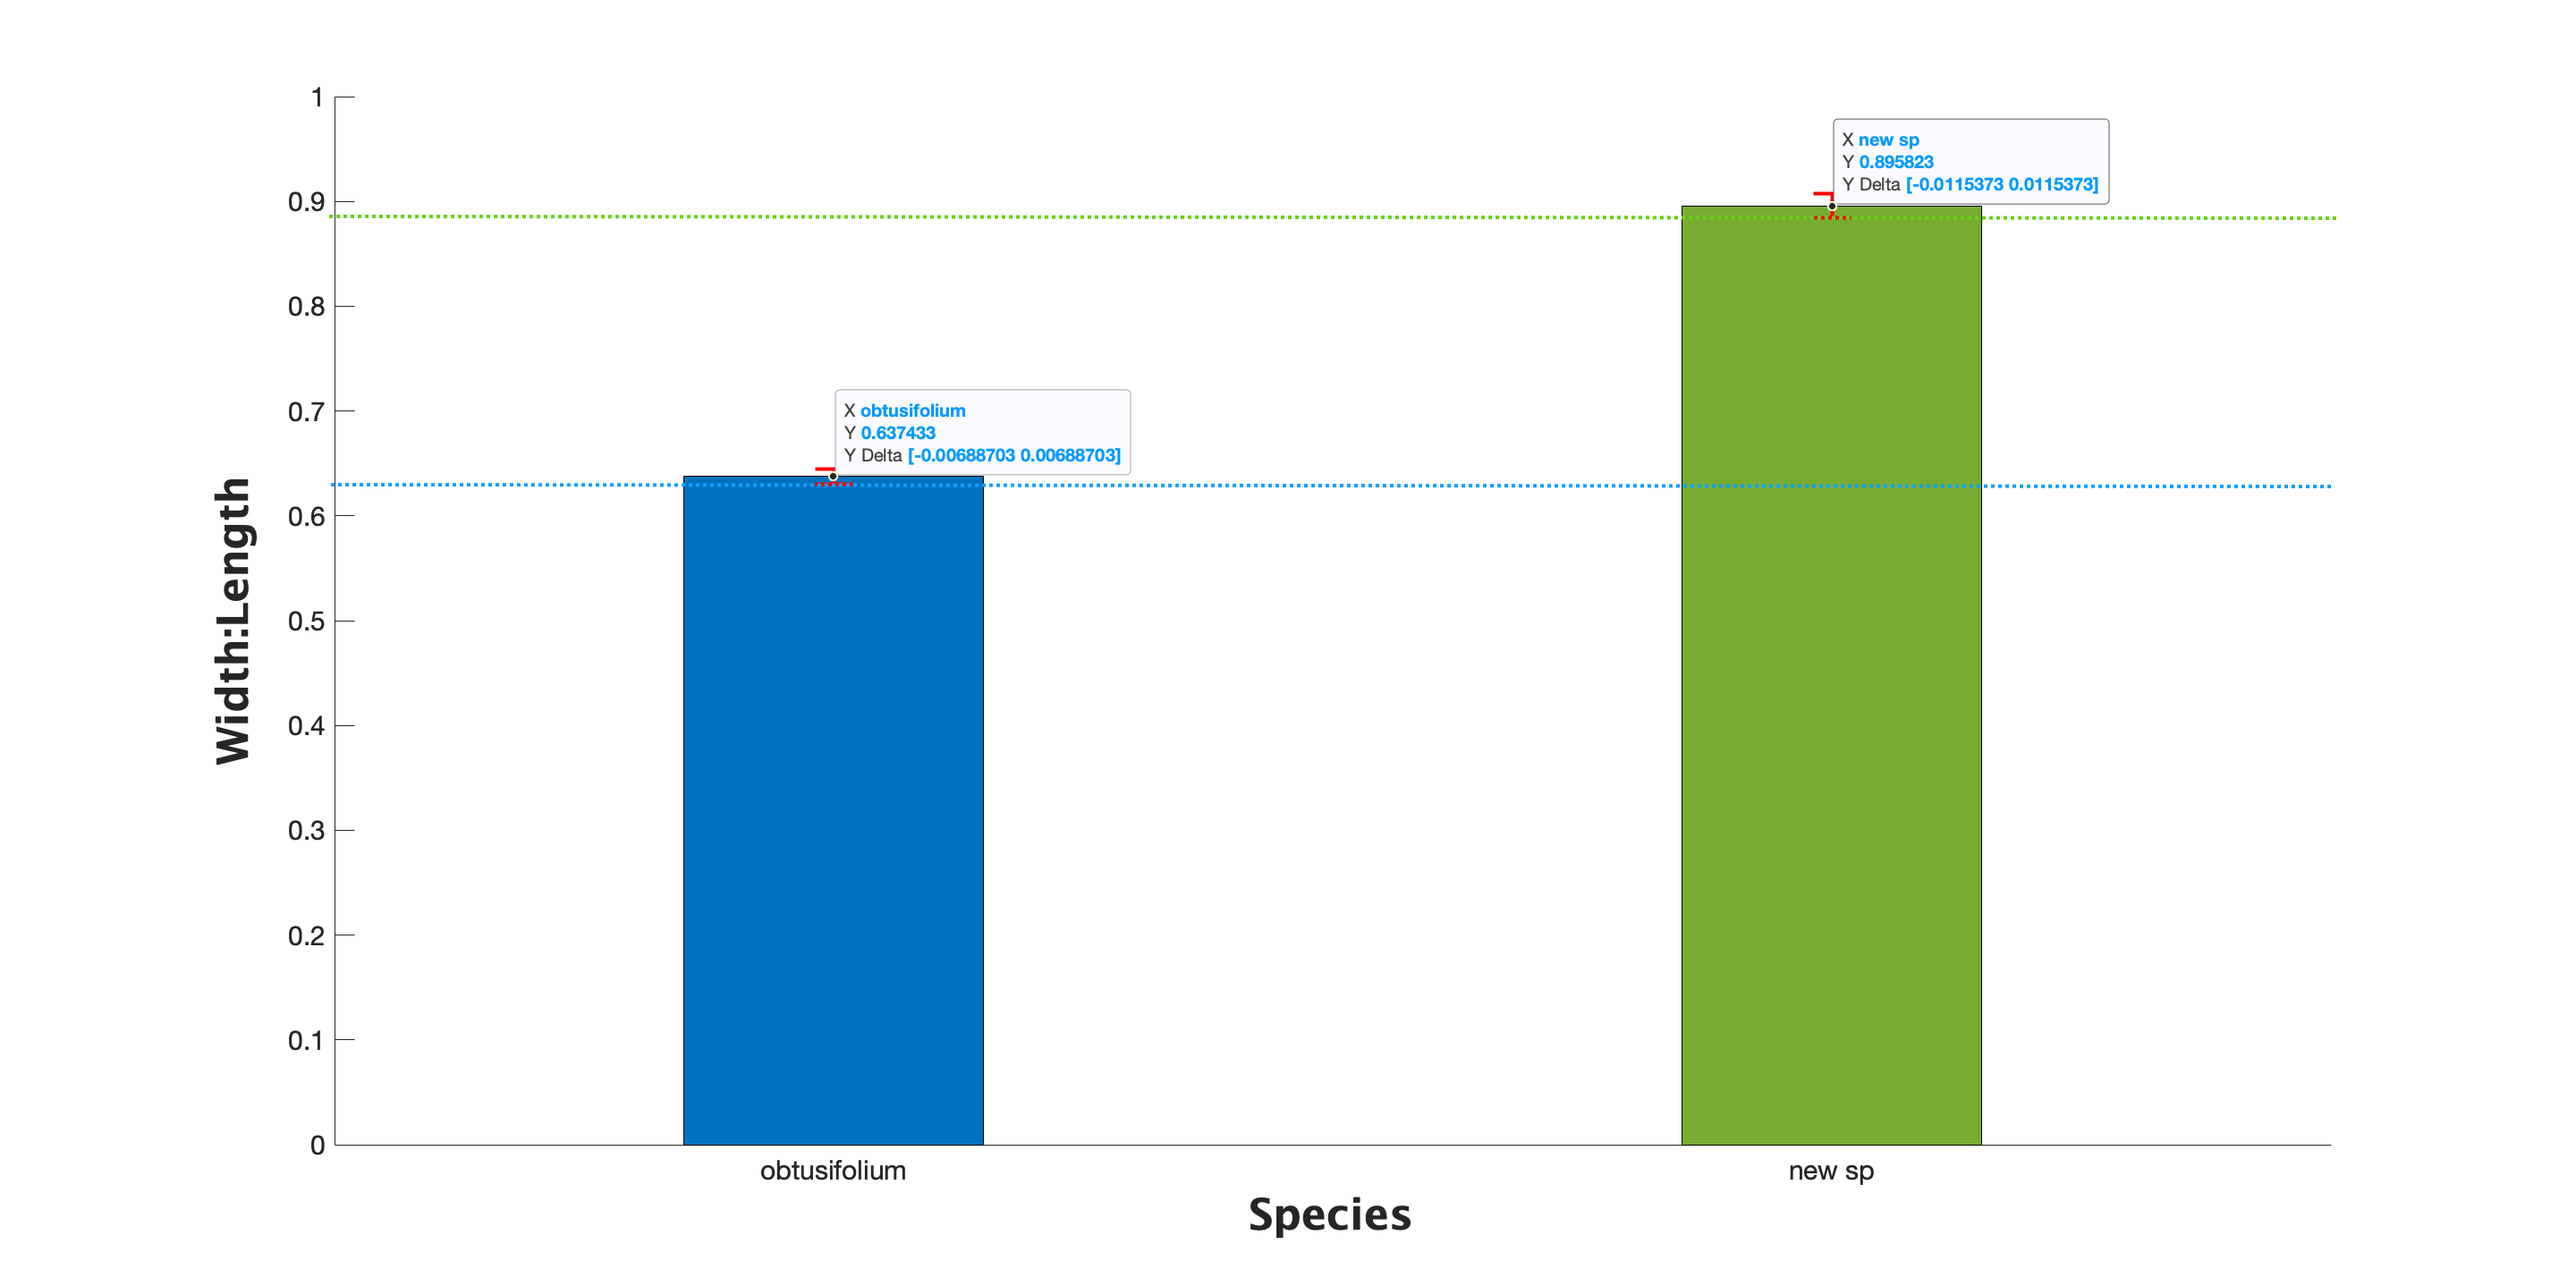
\includegraphics[width=\textwidth]{lab5.png}
  \fbox{\begin{minipage}{45em}
    In the bar chart above, are the length-to-width ratios for Scleropodium obtusifolium and Scleropodium possible new-sp. As you can see from both error bars and the dashed lines across with no overlaps, we can conclude that there is a statistical significant difference meaning the populations represent different species.
  \end{minipage}}
\end{center}
\end{document}
